\documentclass[10pt]{article}
\usepackage[a4paper,margin=17mm]{geometry}
\usepackage{graphicx,hyperref,amsmath,amssymb,array}
\hypersetup{colorlinks=true,urlcolor=blue}
\setlength{\parindent}{0pt}
\setlength{\parskip}{5pt}
\begin{document}
\begin{center}\Large Curve25519: four-point torus construction\\[3pt]
\normalsize 15 November 2026 --- producer evidence, PCC unverified\end{center}

The native Rust compiler constructs an actual-field four-point system with
454 variables and 455 quadratic constraints. A known witness satisfies all
constraints, and all eight raw sections of its prime target are checked.
No large-base solver was invoked. [pcc:unverified]

\begin{center}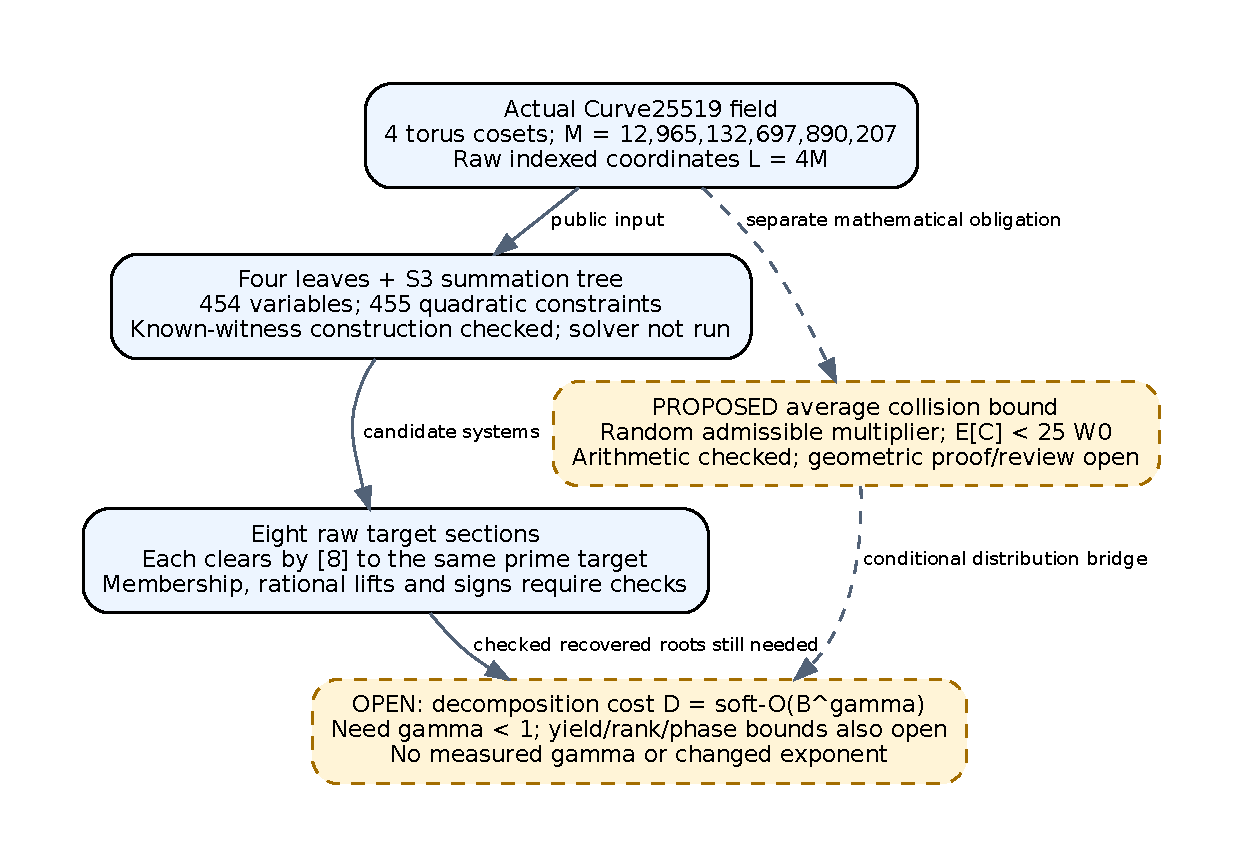
\includegraphics[width=0.94\linewidth,height=112mm,keepaspectratio]{pipeline.pdf}\end{center}

\textbf{Exact instance.}
$E:v^2=u^3+486662u^2+u$, $p=2^{255}-19$,
$\#E(\mathbb F_p)=8\ell$ as sourced from RFC 7748,
$\ell=2^{252}+27742317777372353535851937790883648493$.
The candidate base uses four cosets of a norm-one-torus subgroup of order
$M=60824497\cdot213156431$ in $\mathbb F_{p^2}=\mathbb F_p[\sqrt2]$.
The raw indexed size is $L=4M$; the proposed prime sign-class bound is
$(M-1)/2\le B\le L$, using the stated injection and cofactor-fiber argument.
[pcc:unverified]

\textbf{Controls and their scope.}
The archive \texttt{four-point-v1/} contains public inputs, native scripts,
known points, pre/post records, eight cofactor sections and three native
identity certificates. Exact integer expansion checks the S3 coordinate
identity and both elliptic-map equations. Native construction checks cover
mutations, internal identity sums, arities 2--6 and admissible shifts.
These checks do not prove morphism degrees or solving cost. Inherited
identity/SHA unit tests are separate regressions. PCC-20261115-02fa5a.
[pcc:unverified]

The older 395-variable/396-equation circuit uses three leaves, one coset and
a different $M$. Counts across these constructions are not a speed comparison.
The original report remains historical. No canonical performance edge is added.
[pcc:unverified]

\newpage
\begin{center}\Large Distribution argument and cost target\end{center}
\textbf{Proposed average-energy step.}
For an admissible random torus multiplier $\sigma$, let $r_\sigma(Q)$ count
signed ordered four-tuples of distinct raw indices summing to $Q$ after
cofactor clearing. Define
\[
 W_0=16L(L-1)(L-2)(L-3),\quad
 C_\sigma=\sum_Q r_\sigma(Q)^2,\quad K=2^{28}.
\]
The frozen draft proposes
\[
 \mathbb E_\sigma C_\sigma\le24W_0+
       \frac{K W_0^2}{p+1-28M}<25W_0.
\]
Its cover independence, projective maps, total degree and collision-count
steps require independent review and formalization. This average does not
certify the fixed multiplier-one base. PCC-20261115-1ea4c1. [pcc:unverified]

The Core-only Lean instance proves $M\mid p+1$, $28M<p+1$,
$KW_0<p+1-28M$ and $2^{52}<(M-1)/2$.
The maintained proof gate passed four declarations with zero trusted-native
exceptions; their axiom audit is empty. These are arithmetic dependencies,
not a proof of the proposed geometric bound. PCC-20261115-2deca4.
[pcc:unverified]

If the energy bound holds, weighted Cauchy--Schwarz would transfer a
label-hidden planted hit rate $s$ to uniform-target yield
$y\ge s^2W_0^2/(\ell C_\sigma)$. The oracle must receive only the public
target and base. Constant planted success is still unestablished for the
large system. [pcc:unverified]

\textbf{Conditional exponent target.}
With $D=\widetilde O(B^\gamma)$, relation cost
$\widetilde O(\ell D/B^3)$ and sparse linear algebra
$\widetilde O(B^2)$ balance at exponent $2/(5-\gamma)$.
For $\gamma=0,1/2,1$ this gives $2/5,4/9,1/2$, respectively.
These are hypothetical consequences, not measurements. Need $\gamma<1$,
independent-row/rank and distribution hypotheses, a growing admissible
family, and complete setup/indexing/validation/transport/descent bounds.
[pcc:unverified]

\textbf{When to reject a route.}
The consumer criteria distinguish a checked theorem excluding an explicit
claim, a counterexample to a universal claim, and a preregistered corrected
test rejecting a finite budgeted probability promise. Timeout or OOM parks
that solver at that budget. Failed controls invalidate the experiment.
Finite scaling data do not prove an asymptotic lower bound.

\textbf{Evidence and next work.}
Source-linked \texttt{REPORT.md} links every archive, proof map, receipt and
named obstruction. Generic four-point recovery must check membership,
rational lifts, signs and the actual affine sum. Full-base solving still
needs a qualified isolated Singular runner and live budget/capacity readback;
no cloud job was launched. The broad root library check is preserved as
incomplete after 51 minutes, not a pass. [pcc:unverified]

\textbf{Primary sources.}
\href{https://www.rfc-editor.org/rfc/rfc7748}{RFC 7748};
\href{https://www.rfc-editor.org/rfc/rfc9380}{RFC 9380};
\href{https://people.maths.ox.ac.uk/petit/files/16PKC_primeECDLP.pdf}{Petit--Kosters--Messeng};
\href{https://www.jmilne.org/math/CourseNotes/AV.pdf}{Milne, AV \S5, Corollaries 5.3--5.4};
\href{https://www.normalesup.org/~tibouchi/papers/welldistributed.pdf}{Farashahi et al., Theorems 1--3}.
The latter analyzes encoding distributions but does not automatically prove
the small-coset/shared-multiplier statement. Novelty remains unestablished.
\end{document}
